\subsection{SPI-Master}
\label{sec:SPIMaster}

The microcontroller have to share information with the FPGA, and according to the requirements mentioned in section \ref{sec:Primaryrequirements}, this communication has to happen using Serial Peripheral Interface (SPI). The protocol will operate as descriped in section \ref{sec:SPIcommunication}. It is therefore important that this link never will be a bottleneck for the system application. 

The requirements of the minimum bit-rate depends om what data that needs to be send, and how often it needs to send it. Since the PID-controller is placed in the FPGA, the application only needs to update the current position once every 5 ms, which is the minimal delay that freeRTOS can put on a task. 

The length of the messages send is defined by the driver placed in the FPGA. As described in section \ref{sec:Implementation} all messages will have the length of 14 bits. Updating both pan and tilt requires two messages. Considering all other messages but the main pulling sequence as negligible results in a total bitrate of:

\begin{equation}
Bitrate = \frac{
14 bit * 2	
}{
0.05s
} = 5.600 bit/sec 
\end{equation}

The Cortex M4 have a build in freescale spi module, that supports four different variations of spi, se appendix \ref{sec:CortexM4Datasheet}. However, implementing the spi from scratch, gives the highest degree of control over the process, which is prefer in this project. 

% full dreasd task diagram
\begin{figure}
	\centering
	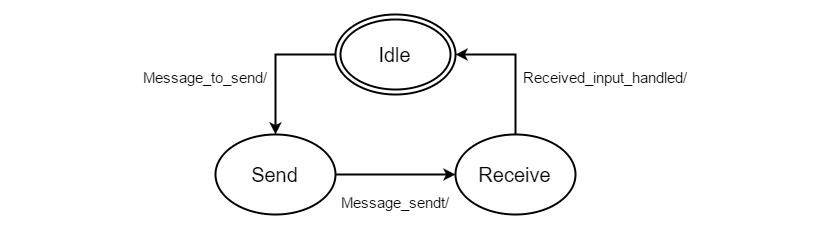
\includegraphics[scale = 0.7] {Billeder/SPI-master}
	\caption{The SPI-master state machine}
	\label{fig:SPI-master}
\end{figure}

The state machine for the task is illustrated in figure \ref{fig:SPI-master}. It consists of three states and is initiated waiting for a message to transmit from the spi\_tx\_queue. When a message is pulled from the queue it jumps to the send state, and after sending the message, the received message will be handled by the P\&T API in the Receive task. From here it will only switch back to the idle state if the API call was successful, else it will continue till it succeeds. 


\subsubsection{Performance Test} 
\label{sec:PerformanceTest}
After implementing the the SPI-master task in the final application the max bit-rate was tested by overloading the spi\_tx\_queue, and giving the SPI-master task High priority int the OS. This made the the task perform at maximum capacity. The measurements of the SPI connection can be seen in figure \ref{fig:HightPerformance}. Since it is able to transmit messages of 14 bots at 7.7 kHz the bitrate will be the product of these two values giving the result $107 kbit/sek$


\begin{figure}
	\centering
	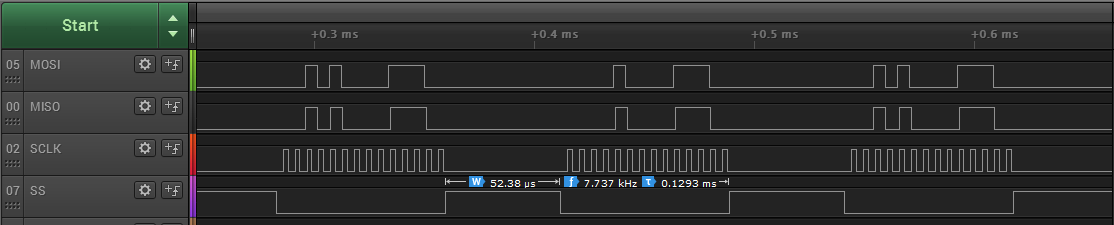
\includegraphics[scale = 0.7] {Billeder/HightPerformance}
	\caption{Shows the max performance of the SPI-Master task}
	\label{fig:HightPerformance}
\end{figure}
 

 